\documentclass[12pt,a4paper]{article}
\usepackage[utf8]{inputenc}
\usepackage[english]{babel}
\usepackage{graphicx}
\usepackage{float}
\usepackage{amsmath}
\usepackage{hyperref}
\usepackage{booktabs}
\usepackage{geometry}
\geometry{margin=1in}

\title{ToolWindow Usage Data Analysis\\Statistical Report}
\author{Data Analysis Project}
\date{\today}

\begin{document}

\maketitle

\begin{abstract}
This report presents a statistical analysis of tool window usage patterns in an IDE environment. The objective is to determine whether there is a significant difference in session duration between tool windows opened manually (via shortcuts, menus, or icons) and those opened automatically (triggered by events such as debugging or test failures). The analysis employs non-parametric statistical tests and effect size measurements to evaluate the practical significance of observed differences.
\end{abstract}

\section{Introduction}

\subsection{Background}
In modern IDEs, tool windows provide quick access to specific tasks or information without requiring users to leave the editor. Users can open these windows through two distinct methods:
\begin{itemize}
    \item \textbf{Manual}: Explicitly opened by the user via keyboard shortcuts, menu selections, or toolbar icons
    \item \textbf{Automatic}: Triggered by system events such as starting a debug session or encountering test failures
\end{itemize}

\subsection{Research Question}
Is there a statistically significant difference in tool window session duration between manual and automatic opening methods?

\subsection{Hypothesis}
\begin{itemize}
    \item $H_0$ (null hypothesis): There is no difference in duration between manual and auto groups
    \item $H_1$ (alternative hypothesis): There is a significant difference in duration between the groups
\end{itemize}

\section{Data Description}

\subsection{Dataset Structure}
The dataset consists of event logs tracking tool window activity with the following fields:
\begin{itemize}
    \item \texttt{user\_id}: Anonymized user identifier (integer)
    \item \texttt{timestamp}: Event time in epoch milliseconds (integer)
    \item \texttt{event}: Event type — either ``opened'' or ``closed''
    \item \texttt{open\_type}: Opening method — ``manual'' or ``auto'' (only present on open events)
\end{itemize}

\subsection{Data Quality Issues}
As with most real-world datasets, the data contains various anomalies:
\begin{itemize}
    \item Close events without prior open events
    \item Multiple consecutive open events without intervening closes
    \item Open events without matching close events
    \item Out-of-order timestamps
    \item Missing or null type values
    \item Negative durations (close timestamp < open timestamp)
\end{itemize}

\section{Methodology}

\subsection{Data Processing Pipeline}

\subsubsection{Step 1: Data Loading}
Raw CSV data is imported into a SQLite database using a multithreaded producer-consumer pattern:
\begin{enumerate}
    \item Producer thread reads CSV file and validates rows
    \item Worker threads parse and normalize event data
    \item Writer thread performs batch insertions into the \texttt{events} table
\end{enumerate}

\subsubsection{Step 2: Data Cleaning}
The cleaning process reconstructs complete usage episodes by matching open/close event pairs per user:

\textbf{Matching Algorithm:}
\begin{enumerate}
    \item Sort events by user ID and timestamp chronologically
    \item For each user, maintain a state machine tracking the current open event
    \item Match each close event with its corresponding open event
    \item Validate timestamp ordering and duration constraints
    \item Filter anomalies into a separate \texttt{anomaly} table
    \item Store clean episodes in the \texttt{clear} table
\end{enumerate}

\textbf{Anomaly Detection Rules:}
\begin{itemize}
    \item \texttt{missing\_open}: Close event without prior open
    \item \texttt{missing\_close}: Open event without matching close
    \item \texttt{duplicate\_open}: Multiple opens without intervening close
    \item \texttt{null\_type}: Open event with missing type
    \item \texttt{closed\_not\_null\_type}: Close event with non-null type
    \item \texttt{out\_of\_order}: Timestamp ordering violation
    \item \texttt{negative\_duration}: Close timestamp precedes open timestamp
    \item \texttt{>duration}: Episode duration exceeds threshold (default: 720 minutes)
\end{itemize}

\subsubsection{Step 3: Duration Calculation}
For each clean episode, calculate duration in minutes:
\begin{equation}
    \text{duration} = \frac{\text{close\_timestamp} - \text{open\_timestamp}}{60000}
\end{equation}

Episodes are grouped by \texttt{type} (manual vs. auto) for comparative analysis.

\subsection{Statistical Analysis}

\subsubsection{Descriptive Statistics}
For each group (manual and auto), compute:
\begin{itemize}
    \item Count (sample size)
    \item Mean duration
    \item Median duration
    \item Standard deviation
    \item Quartiles (Q1, Q3)
    \item Interquartile range (IQR)
\end{itemize}

\subsubsection{Mann-Whitney U Test}
A non-parametric test chosen for the following reasons:
\begin{itemize}
    \item No assumption of normal distribution (common for duration data)
    \item Robust to outliers
    \item Suitable for comparing two independent samples
    \item Tests whether distributions differ in location (central tendency)
\end{itemize}

\textbf{Significance Level:} $\alpha = 0.05$

\textbf{Decision Rule:}
\begin{itemize}
    \item If $p < 0.05$: Reject $H_0$, conclude significant difference exists
    \item If $p \geq 0.05$: Fail to reject $H_0$, insufficient evidence of difference
\end{itemize}

\subsubsection{Effect Size: Cliff's Delta}
To quantify the magnitude of difference, we compute Cliff's Delta ($\delta$):

\begin{equation}
    \delta = \frac{\#(x > y) - \#(x < y)}{n_1 \cdot n_2}
\end{equation}

where $x \in \text{Manual}$, $y \in \text{Auto}$, and $n_1, n_2$ are sample sizes.

\textbf{Interpretation Guidelines:}
\begin{itemize}
    \item $|\delta| < 0.15$: Negligible effect
    \item $0.15 \leq |\delta| < 0.33$: Small effect
    \item $0.33 \leq |\delta| < 0.47$: Medium effect
    \item $|\delta| \geq 0.47$: Large effect
\end{itemize}

\subsection{Visualization}
Three types of plots are generated:
\begin{enumerate}
    \item \textbf{Histogram}: Distribution comparison of durations
    \item \textbf{Box Plot}: Quartile and outlier visualization
    \item \textbf{Violin Plot}: Density distribution comparison
\end{enumerate}

\section{Results}

\subsection{Data Summary}
\begin{itemize}
    \item Total raw events loaded: [REPLACE WITH ACTUAL]
    \item Clean episodes reconstructed: [REPLACE WITH ACTUAL]
    \item Manual episodes: [REPLACE WITH ACTUAL]
    \item Auto episodes: [REPLACE WITH ACTUAL]
    \item Anomalies filtered: [REPLACE WITH ACTUAL]
\end{itemize}

\subsection{Descriptive Statistics}

\begin{table}[H]
\centering
\caption{Descriptive Statistics by Opening Type}
\begin{tabular}{@{}lrr@{}}
\toprule
\textbf{Statistic} & \textbf{Manual} & \textbf{Auto} \\
\midrule
Count & [REPLACE] & [REPLACE] \\
Mean (min) & [REPLACE] & [REPLACE] \\
Median (min) & [REPLACE] & [REPLACE] \\
Std Dev (min) & [REPLACE] & [REPLACE] \\
Q1 (min) & [REPLACE] & [REPLACE] \\
Q3 (min) & [REPLACE] & [REPLACE] \\
IQR (min) & [REPLACE] & [REPLACE] \\
\bottomrule
\end{tabular}
\end{table}

\subsection{Statistical Test Results}

\textbf{Mann-Whitney U Test:}
\begin{itemize}
    \item U-statistic: [REPLACE WITH ACTUAL]
    \item p-value: [REPLACE WITH ACTUAL]
    \item Conclusion: [REPLACE: Reject/Fail to reject $H_0$]
\end{itemize}

\textbf{Effect Size (Cliff's Delta):}
\begin{itemize}
    \item $\delta$: [REPLACE WITH ACTUAL]
    \item Magnitude: [REPLACE: negligible/small/medium/large]
    \item Interpretation: [REPLACE: Manual durations are lower/higher than Auto]
\end{itemize}

\subsection{Visualizations}

\begin{figure}[H]
    \centering
    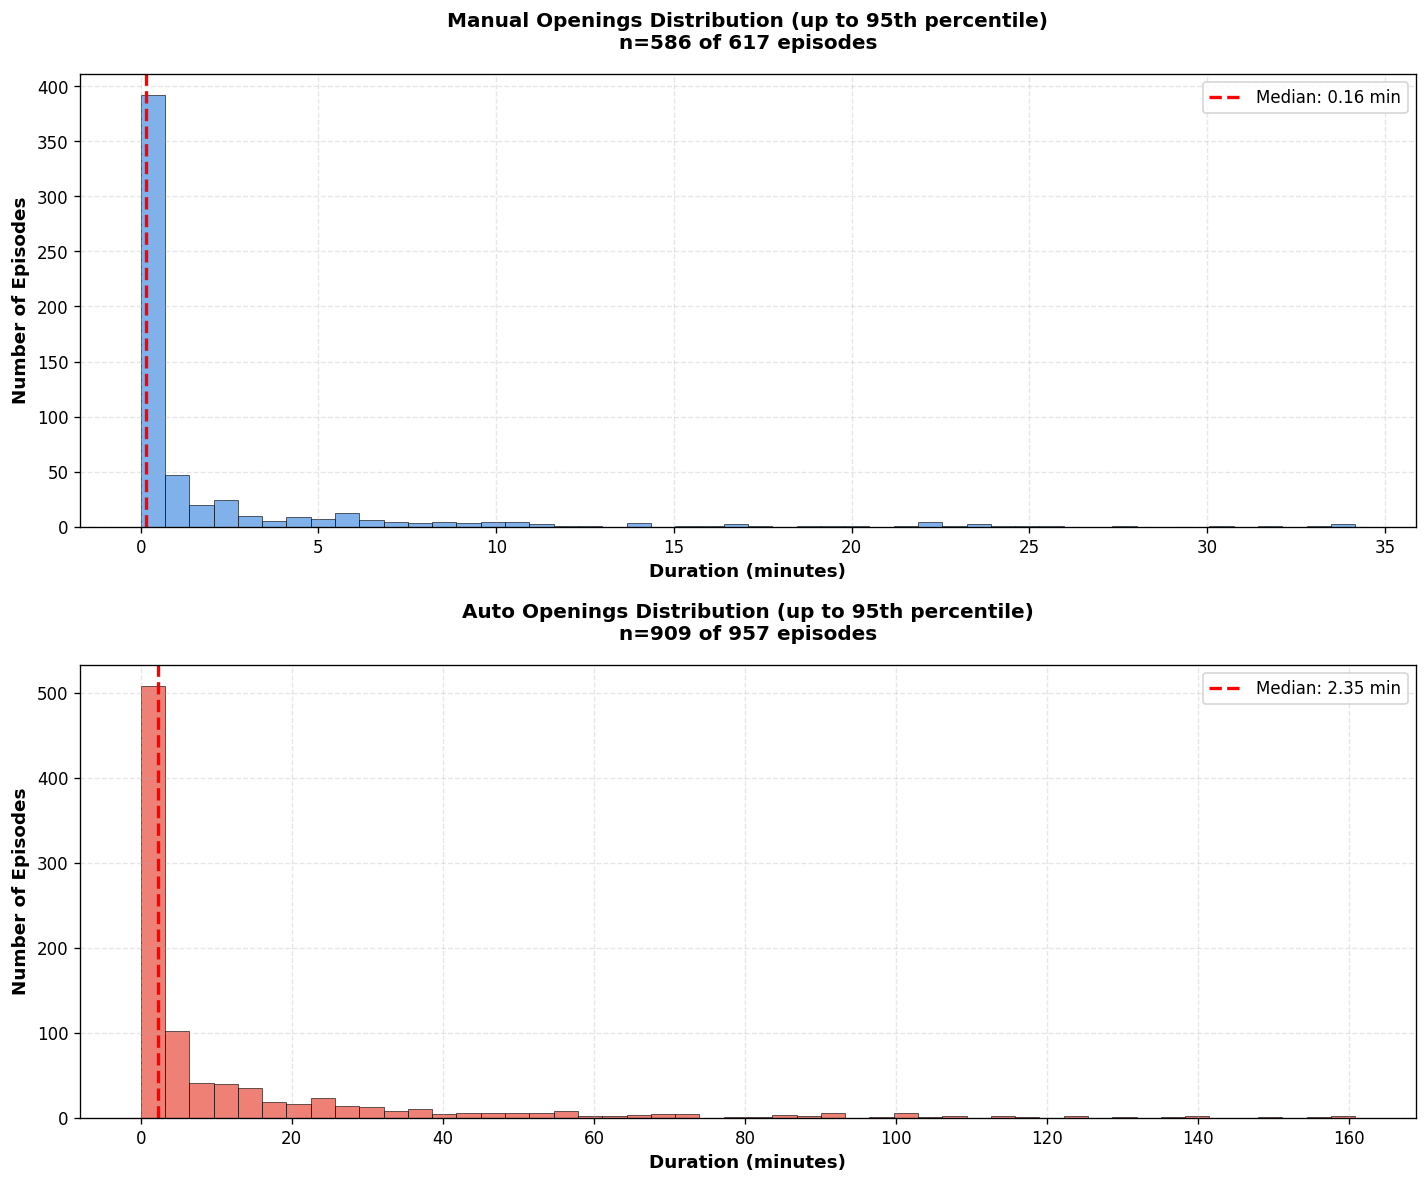
\includegraphics[width=0.8\textwidth]{plots/histogram.png}
    \caption{Duration Distribution Comparison (Histogram)}
\end{figure}

\begin{figure}[H]
    \centering
    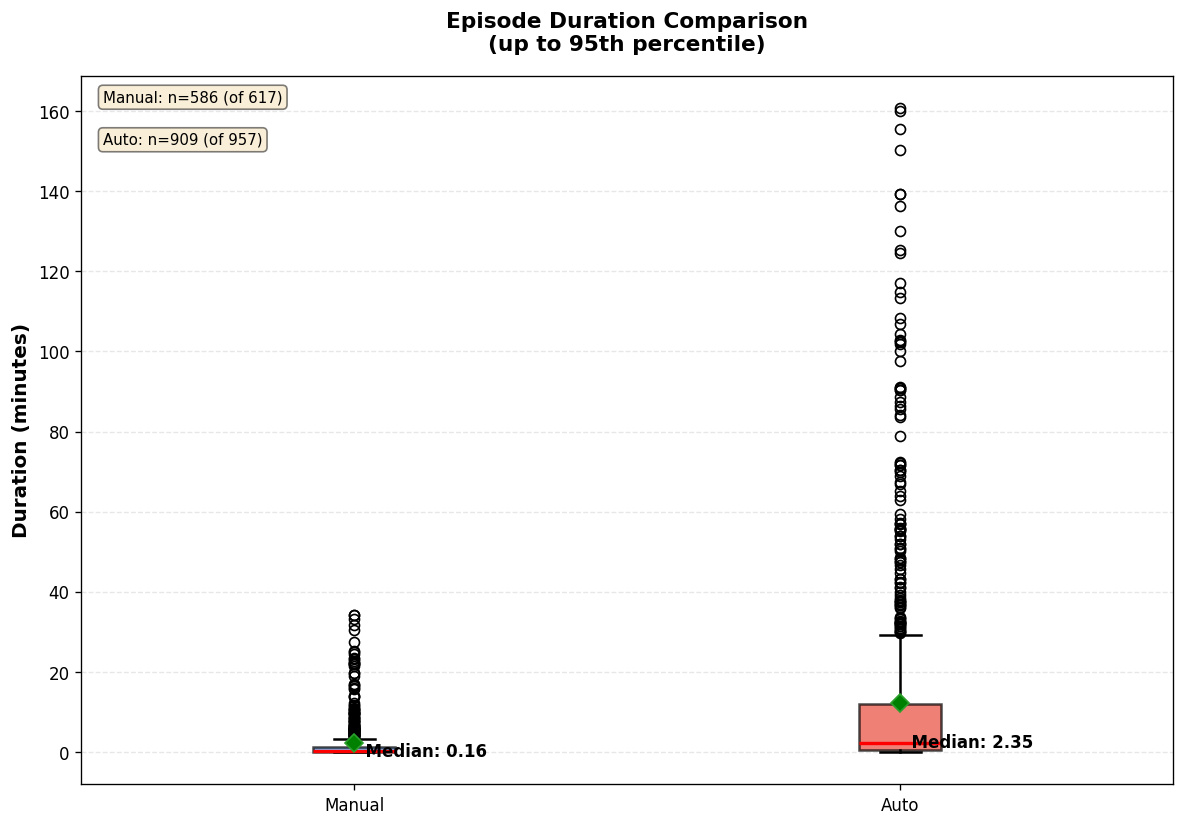
\includegraphics[width=0.8\textwidth]{plots/boxplot.png}
    \caption{Duration Distribution Comparison (Box Plot)}
\end{figure}

\begin{figure}[H]
    \centering
    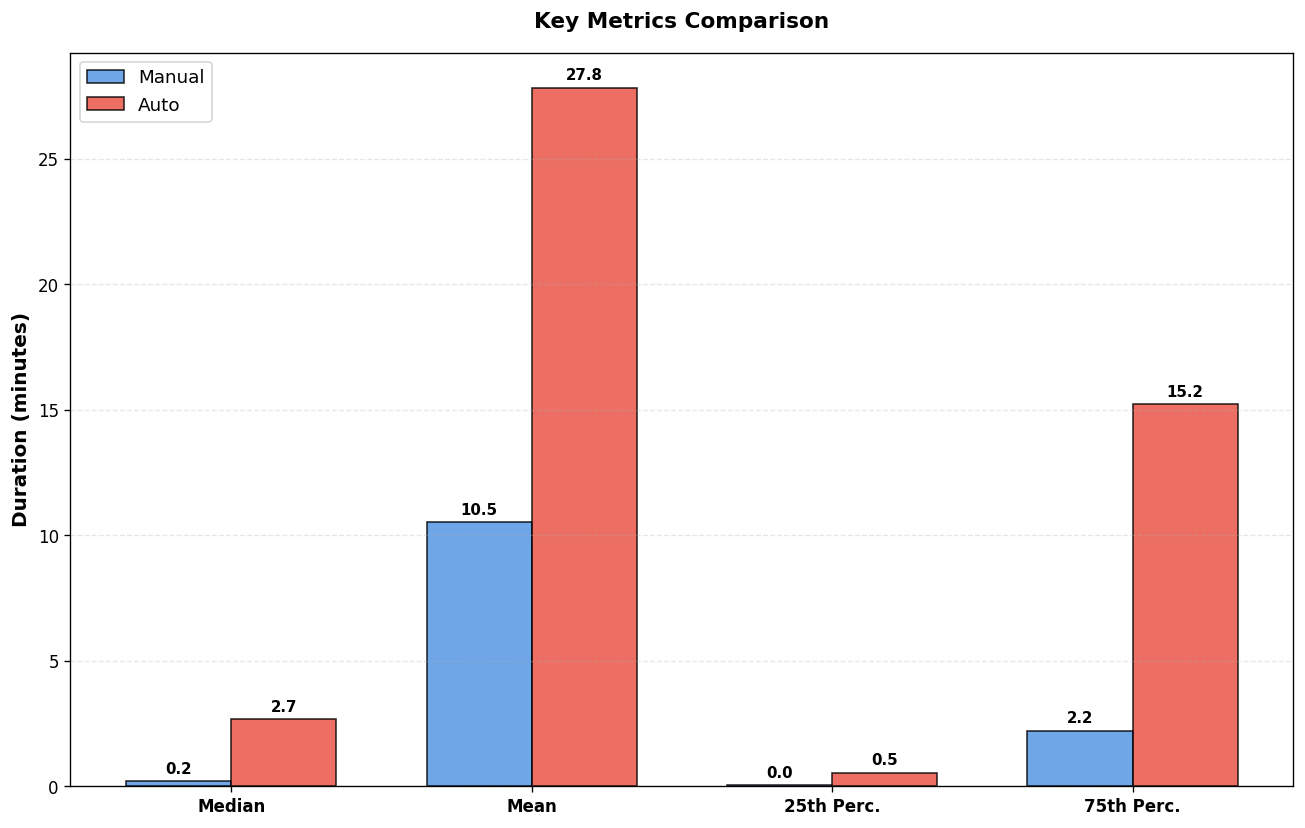
\includegraphics[width=0.8\textwidth]{plots/comparison.png}
    \caption{Side-by-Side Distribution Comparison}
\end{figure}

\section{Discussion}

\subsection{Interpretation of Results}
[REPLACE WITH ACTUAL INTERPRETATION BASED ON YOUR RESULTS]

The analysis reveals [significant/no significant] difference between manual and auto opening methods. The effect size of [REPLACE] indicates a [negligible/small/medium/large] practical difference.

\subsection{Possible Explanations}
Potential reasons for observed patterns:
\begin{itemize}
    \item \textbf{Manual opens}: Users may close windows more quickly when they explicitly open them for specific tasks
    \item \textbf{Auto opens}: System-triggered windows may remain open longer as users complete debugging or testing workflows
    \item \textbf{User intent}: Manual actions reflect deliberate decisions, while auto triggers may not align with immediate user needs
\end{itemize}

\subsection{Limitations}
\begin{itemize}
    \item Anonymized data prevents investigation of individual user patterns
    \item Dataset may not capture all usage contexts
    \item Threshold-based filtering (720 min) may exclude legitimate long sessions
    \item Temporal factors (time of day, day of week) not considered
\end{itemize}

\subsection{Assumptions}
\begin{enumerate}
    \item Episodes exceeding 12 hours are considered anomalous
    \item Events within the same timestamp are ordered with closes before opens
    \item Users operate independently (no correlation between users)
    \item Missing close events indicate incomplete sessions (not system errors)
\end{enumerate}

\section{Conclusions}

Based on the statistical analysis:
\begin{enumerate}
    \item [REPLACE: State whether significant difference was found]
    \item [REPLACE: State the practical significance based on effect size]
    \item [REPLACE: Provide recommendation or insight]
\end{enumerate}

\subsection{Recommendations}
\begin{itemize}
    \item Consider implementing adaptive window behavior based on opening method
    \item Investigate user workflows to understand duration differences
    \item Collect additional context (task type, time of day) for deeper analysis
\end{itemize}

\section{Technical Implementation}

\subsection{Technology Stack}
\begin{itemize}
    \item \textbf{Language}: Python 3.12+
    \item \textbf{Database}: SQLite3
    \item \textbf{Statistical Libraries}: scipy, matplotlib
    \item \textbf{Web Framework}: FastAPI + Jinja2
    \item \textbf{Deployment}: Docker + Docker Compose
\end{itemize}

\subsection{Repository Structure}
\begin{verbatim}
ToolWindowData/
├── run.py              # Main pipeline entry point
├── src/
│   ├── loader.py      # CSV import module
│   ├── janitor.py     # Data cleaning module
│   ├── science.py     # Statistical analysis
│   └── web.py         # Web dashboard
├── database/
│   └── toolwindow.sql # Database schema
└── plots/             # Generated visualizations
\end{verbatim}

\subsection{Reproducibility}
To reproduce the analysis:
\begin{verbatim}
# Clone repository
git clone [repository-url]

# Run with Docker
make all

# Access results
open http://localhost:8000
\end{verbatim}

\section{References}
\begin{itemize}
    \item Mann, H. B., \& Whitney, D. R. (1947). On a test of whether one of two random variables is stochastically larger than the other. \textit{Annals of Mathematical Statistics}, 18(1), 50-60.
    \item Cliff, N. (1993). Dominance statistics: Ordinal analyses to answer ordinal questions. \textit{Psychological Bulletin}, 114(3), 494-509.
    \item Romano, J., et al. (2006). Appropriate statistics for ordinal level data: Should we really be using t-test and Cohen's d for evaluating group differences on the NSSE and other surveys? \textit{Annual meeting of the Florida Association of Institutional Research}, 177.
\end{itemize}

\appendix
\section{SQL Schema}

\subsection{Events Table}
\begin{verbatim}
CREATE TABLE events (
    id INTEGER PRIMARY KEY AUTOINCREMENT,
    user_id INTEGER NOT NULL,
    timestamp INTEGER NOT NULL,
    event TEXT NOT NULL CHECK(event IN ('opened', 'closed')),
    type TEXT CHECK(type IN ('manual', 'auto'))
);
\end{verbatim}

\subsection{Clear Episodes Table}
\begin{verbatim}
CREATE TABLE clear (
    id INTEGER PRIMARY KEY AUTOINCREMENT,
    type TEXT NOT NULL CHECK(type IN ('manual', 'auto')),
    start INTEGER NOT NULL,
    end INTEGER NOT NULL,
    open_event_id INTEGER NOT NULL,
    close_event_id INTEGER NOT NULL
);
\end{verbatim}

\subsection{Anomaly Table}
\begin{verbatim}
CREATE TABLE anomaly (
    id INTEGER PRIMARY KEY AUTOINCREMENT,
    type TEXT,
    timestamp INTEGER NOT NULL,
    related_event_id INTEGER,
    event_id INTEGER NOT NULL,
    detail TEXT NOT NULL
);
\end{verbatim}

\end{document}

